%!TEX program = xelatex
\documentclass[12pt,a4paper,utf8]{ctexart}
\usepackage{graphicx}
\usepackage{amsmath}
\usepackage{amssymb}
\usepackage{subfig}
\usepackage{cite}
\usepackage[ntheorem]{empheq}
\usepackage{enumitem}
\usepackage{fullpage}
\usepackage{cleveref}
\usepackage{cellspace}
\usepackage{listings}
\usepackage{color}
\definecolor{gray}{rgb}{0.5,0.5,0.5}
\definecolor{dkgreen}{rgb}{.068,.578,.068}
\definecolor{dkpurple}{rgb}{.320,.064,.680}

% set Matlab styles
\lstset{
   language=Matlab,
   keywords={break,case,catch,continue,else,elseif,end,for,function,
      global,if,otherwise,persistent,return,switch,try,while},
   basicstyle=\ttfamily,
   keywordstyle=\color{blue}\bfseries,
   commentstyle=\color{dkgreen},
   stringstyle=\color{dkpurple},
   backgroundcolor=\color{white},
   tabsize=4,
   showspaces=false,
   showstringspaces=false
}

\begin{document}
\CJKfamily{zhkai}	


\begin{center}
\textbf{作业二}\\
\textbf{林成渊 ~~~~~ PB18051113 ~~~~~ \zhtoday}\\
\end{center}
\textit{}
\vspace{\baselineskip}

\begin{enumerate}
\item[第一题] \textbf{使用多种方法计算积分}

(a)根据题意,编写代码使用自动控制误差的复化梯形公式计算积分
\begin{lstlisting}[frame=single]
clear, clc, clf
MS = 'MarkerSize'; ms = 8;
MC = 'MarkerFaceColor';

% Def of the problem
F = @(x) sin(cos(sin(cos(x))));
a = -1; b = 1;
tol = 1e-15;


%%
% Init the Loop
n = 1; % Initial of the intervals

h = (b - a) / n;
x = linspace(a, b, n + 1);
% Save each Int value, Dynamic Programming
I = zeros(1, 100);
I(2) = h * (F(a) / 2 + sum(F(x(2:end - 1))) + F(b) / 2);
I(1) = I(2)+1;
i = 2;
% Loop begin
while abs(I(i) - I(i-1)) > 3*tol
    % If this loop begin, the former loop failed
    % Switch to a new loop
    i = i + 1;
    h = h / 2; 
    % Calculate for this loop
    H = h * sum(F(a + (2 * (1:n) - 1) * h));
    I(i) = I(i-1)/2 + H;
    
    n = n * 2;
end
%%
% Output
format long
display(I(i));
display(n);
figure(1);
semilogy((1:i-1), abs(I(2:i) - I(i))/3, 'ro-', MC, 'b', MS, ms);
xlabel('迭代次数');
ylabel('误差');
\end{lstlisting}
输出结果,积分值为1.339880713117285,使用插值点数为16777216。得到图1
\begin{figure}[htbp]
    \centering
    \includegraphics[width=0.7\textwidth]{image/T1_a.eps}
    \caption{第一题(a)小题作图结果}
\end{figure}

(b)根据题意,编写代码使用Richardson外推方法计算积分,代码如下
\begin{lstlisting}[frame=single]
clear , clc , clf
MS = 'MarkerSize'; ms = 8;
MC = 'MarkerFaceColor';

% Def of the problem
F = @(x) sin(cos(sin(cos(x))));
a = -1; b = 1;
tol = 1e-15;

% Some other options
M = 15;

%%
% Init the Loop
R = zeros(M,M);
n = 1; % Initial of the intervals
h = b - a;
R(1,1) = (F(a) + F(b)) * h / 2;
errors = zeros(M-1);
for k = 2:M
    R(k,1) = (R(k-1,1) +
            h*sum(F(a + (2.*(1:n)-1) .* (h/2)))) / 2;
    h = h / 2;
    n = n * 2;
    for j = 2:k
        R(k,j) = R(k,j-1) +
                (R(k,j-1) - R(k-1,j-1))/(4^(j-1) - 1);
    end
    errors(k-1) = abs(R(k,k)-R(k-1,k-1));
    if errors(k-1) < tol
        break;
    else
    end
end

%%
% Output
format long
disp(R(k,k));
disp(k-1);
figure(1);
semilogy((1:k-1), errors(1:k-1), 'ro-', MC, 'b', MS, ms);
xlabel('迭代次数');
ylabel('误差');
\end{lstlisting}
输出结果,积分值为1.339880713117284,使用插值点数为$2^8 = 256$。得到图2
\begin{figure}[htbp]
    \centering
    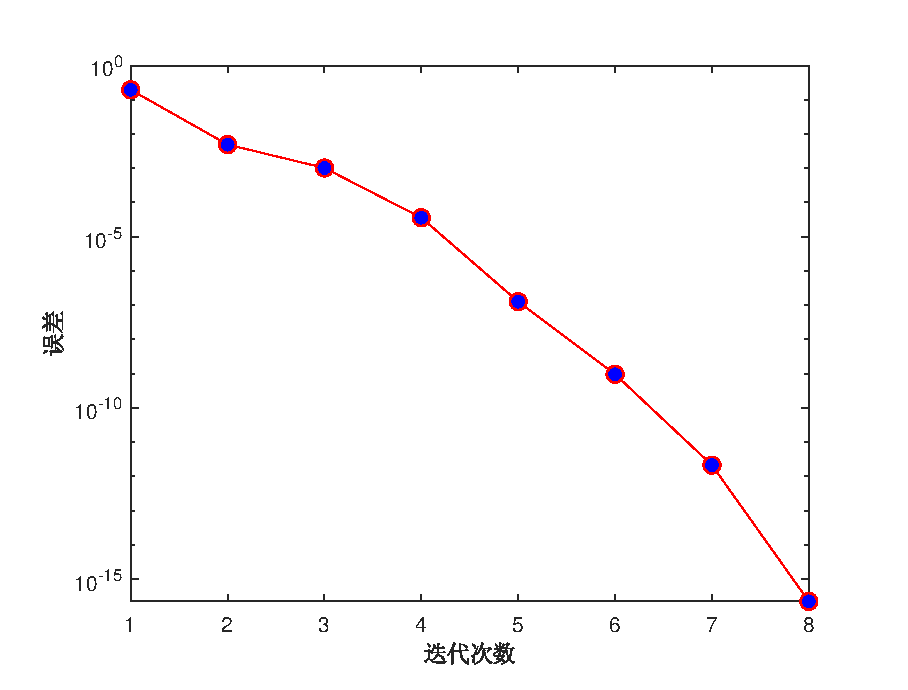
\includegraphics[width=0.7\textwidth]{image/T1_b.eps}
    \caption{第一题(b)小题作图结果}
\end{figure}

(c)根据题意,编写代码使用Gauß积分方法计算积分,代码如下
\begin{lstlisting}[frame=single]
clear,clc
LW = 'LineWidth'; lw = 2;
MS = 'MarkerSize'; ms = 8;
MC = 'MarkerFaceColor';

% Def of the problem
F = @(x) sin(cos(sin(cos(x))));
a = -1; b = 1;
tol = 1e-15;

% Other Options
M = 20;
I = zeros(1,M);
[x, w] = gauss(1);
I(1) = w*F(x);
errors = zeros(1,M-1);
for n = 2:M
    [x,w] = gauss(n);
    I(n) = w*F(x);
    errors(n-1) = abs(I(n) - I(n-1));
    display(errors(n-1));
    if abs(I(n)-I(n-1)) < tol
        break;
    else
    end
end
%%
% Output
format long
disp(I(n));
disp(n);
figure(1);
semilogy((2:n), errors(1:n-1), 'ro-', MC, 'b', MS, ms);
xlabel('n的取值');
ylabel('误差');

% GAUSS  nodes x (Legendre points) and weights w
%        for Gauss quadrature

function [x,w] = gauss(N)
    beta = .5./sqrt(1-(2*(1:N-1)).^(-2));
    T = diag(beta,1) + diag(beta,-1);
    [V,D] = eig(T);
    x = diag(D); [x,i] = sort(x);
    w = 2*V(1,i).^2;
end
\end{lstlisting}
输出结果,积分值为1.339880713117284,得出这个积分本身使用了15个插值点,每次迭代使用的插值点数及其误差如图3
\begin{figure}[htbp]
    \centering
    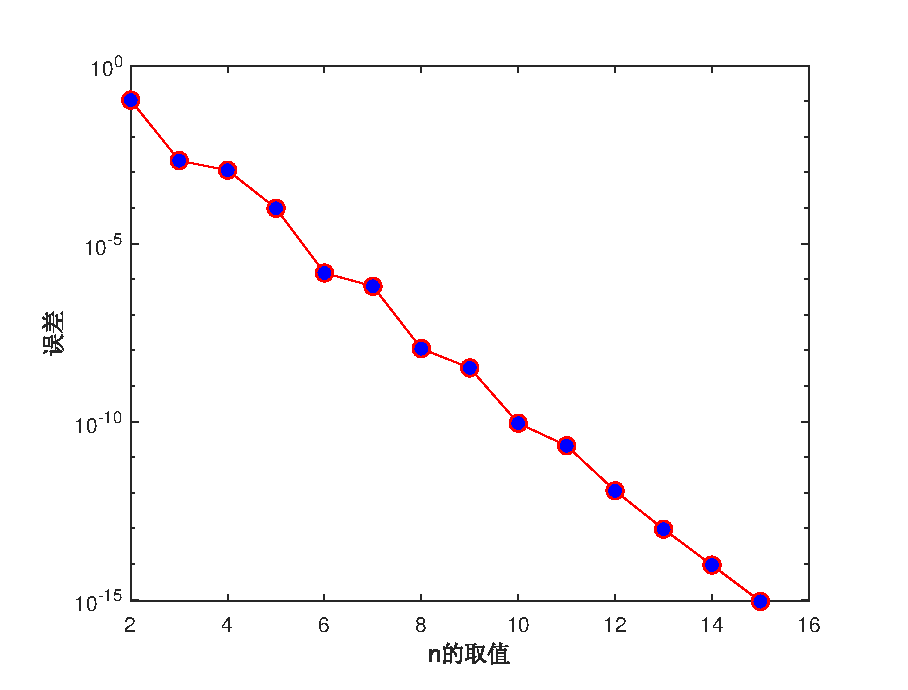
\includegraphics[width=0.7\textwidth]{image/T1_c.eps}
    \caption{第一题(c)小题作图结果}
\end{figure}

(d)以上三种方法计算积分均以接近计算机的机器精度为其迭代的目标误差上界。
最后,使用自动控制误差的复化梯形公式总共采样16777216个点,
使用Richardson外推方法计算积分总共采样256个点,
使用Gauß积分方法计算积分总共采样15个点,
由此可见,就效率而言,三种方法从高到低依次排序为:
Gauß积分方法、Richardson外推方法、使用自动控制误差的复化梯形公式方法。

\item[第二题] \textbf{函数求导与微分矩阵(differentiation matrix)}

(a)证明:根据题设条件得
\begin{equation}
    \begin{aligned}
        \ell_j'(x) &= (\frac{1}{\pi_j} \prod_{k=0,k\neq j}^n (x-x_k))' \\
                    &= \frac{1}{\pi_j} (\prod_{k=0,k\neq j}^n (x-x_k))' \\
                    &= \frac{1}{\pi_j} ( (x-x_1)(x-x_2)\dots (x-x_n) + (x-x_0)(x-x_3)\dots (x-x_n) + \dots ) \\
                    &= \frac{1}{\pi_j} ( \frac{\prod_{k=0,k\neq j}^n (x-x_k)}{x-x_0} + \frac{\prod_{k=0,k\neq j}^n (x-x_k)}{x-x_1} + \dots + \frac{\prod_{k=0,k\neq j}^n (x-x_k)}{x-x_n} ) \\
                    &= \frac{1}{\pi_j} \prod_{k=0,k\neq j}^n (x-x_k) *(\frac{1}{x-x_0} + \frac{1}{x-x_1} + \dots) \\
                    &= \frac{1}{\pi_j} \prod_{k=0,k\neq j}^n (x-x_k) *\sum_{k=0,k\neq j}^n \frac{1}{x-x_k} \\
                    &= \ell_j(x) \sum_{k=0,k\neq j}^n (x-x_k)^{-1}
    \end{aligned}
    \nonumber
\end{equation}
所以有
\begin{equation}
    \begin{aligned}
        p'(x) &= \sum_{j=0}^n f_j\ell'_j(x) \\ 
                &= \sum_{j=0}^n \bigg(f_j\ell_j(x)\sum_{k=0,k\neq j}^n(x-x_k)^{-1}\bigg)
    \end{aligned}
    \nonumber
\end{equation}
(b)根据题设编写matlab代码进行实现
\begin{lstlisting}[frame=single]
clear, clc, clf
LW = 'linewidth'; lw = 2;
%%
%Calculate all the 16 fj
n = 15;
x = linspace(-1, 1, n+1)';
F = @(x)sin(x);
f = F(x);
%%
%Calculate all the 1001 exact value
m = 1000;
xx = linspace(-1, 1, m+1)';
F_divide = @(x)cos(x);
exact = F_divide(xx);
%%
%Calculate all the 1001 approximate value
approx = zeros(m+1, 1);
for j = 1:n+1
    l = ones(m+1, 1);
    div_factor = zeros(m+1,1);
    for k = 1:j-1
         l = l.*(xx - x(k))/(x(j) - x(k));
         div_factor = div_factor + (1./(xx-x(k)));
    end
    for k = j+1:n+1
         l = l.*(xx - x(k))/(x(j) - x(k));
         div_factor = div_factor + (1./(xx-x(k)));
    end
    approx = approx + f(j)*l.*div_factor;
end
%%
%Calculate all the 1001 error
error = abs(exact - approx);
%%
figure(1);
subplot(2,1,1);
p1=plot(xx,exact,'k',LW,lw); hold on
p2=plot(xx,approx,'b--',LW,lw); hold on
legend([p1,p2], 'exact', 'approx');
subplot(2,1,2);
p3=semilogy(xx,error,'b',LW,lw); hold on
legend(p3, 'error','location','se');
\end{lstlisting}
运行得到图4结果
\begin{figure}[htbp]
    \centering
    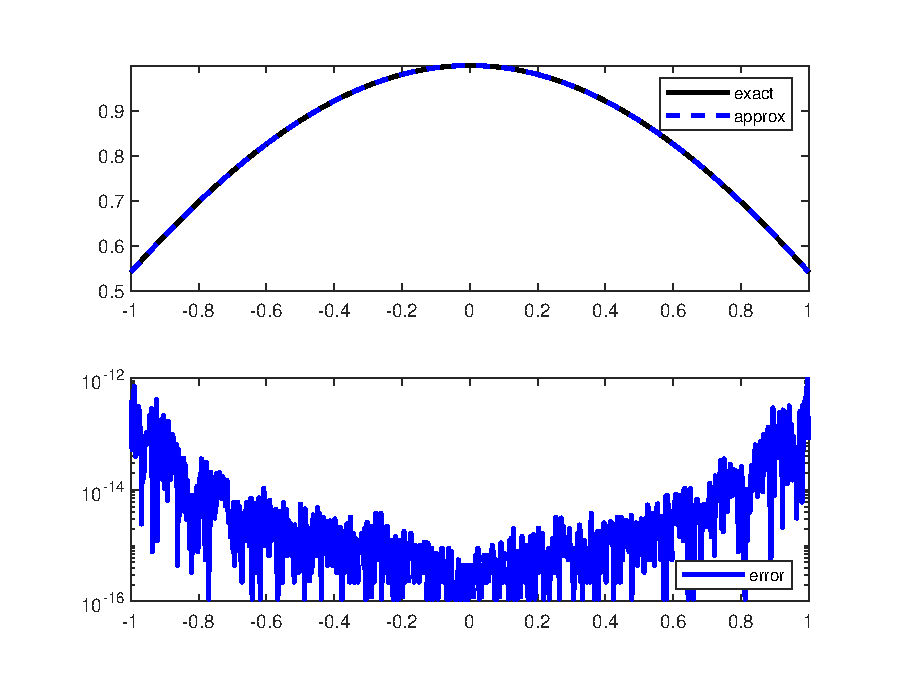
\includegraphics[width=0.7\textwidth]{image/T2_b.eps}
    \caption{第二题(b)小题作图结果}
\end{figure}

(c)由题设分析得
\begin{equation}
    \begin{aligned}
        P'  &=  \left[\begin{matrix}
                    P'(x_0) \\
                    P'(x_1) \\
                    \vdots \\
                    P'(x_n)
                \end{matrix}\right] \\
            &=  \left[\begin{matrix}
                D_{00} & D_{01} & \dots & D_{0n} \\
                D_{10} & D_{11} & \dots & D_{1n} \\
                \vdots & \vdots & \ddots & \vdots \\
                D_{n0} & D_{n1} & \dots & D_{nn}
                \end{matrix}\right] 
                \left[\begin{matrix}
                    f(x_0) \\
                    f(x_1) \\
                    \vdots \\
                    f(x_n)
                \end{matrix}\right] \\
            &=  \left[\begin{matrix}
                \sum_{j=0}^n f_jD_{0j} \\
                \sum_{j=0}^n f_jD_{1j} \\
                \vdots \\
                \sum_{j=0}^n f_jD_{nj}
                \end{matrix}\right]
    \end{aligned}
    \nonumber
\end{equation}
对照式子
\begin{equation}
    p'(x) = \sum_{j=0}^n \bigg(f_j\ell_j(x)\sum_{k=0,k\neq j}^n(x-x_k)^{-1}\bigg) \nonumber
\end{equation}
得到
\begin{equation}
    D_{ij} = \ell_j(x_i) \sum_{k=0,k\neq j}^n (x-x_k)^{-1} \nonumber
\end{equation}
又由
\begin{equation}
    \ell_j(x_k) = \left\{   \begin{aligned}
                                1&\quad k = j \\
                                0&\quad k \neq j
                            \end{aligned}   \right. \nonumber
\end{equation}
有
\begin{equation}
    \begin{aligned}
        D_{ij} &= \ell_j(x_i) \sum_{k=0,k\neq j}^n (x-x_k)^{-1} \\
                &= \left\{   \begin{aligned}
                                0+0+\dots + \ell_j(x_i) \frac{1}{x-x_i} + \dots + 0 
                                = \frac{1}{\pi_j} \prod_{k=0,k\neq i,j}^n(x_i-x_k) 
                                = \frac{\pi_i}{\pi_j(x_i-x_j)} \quad &i\neq j \\
                                \sum_{k=0,k\neq j}^n (x_j-x_k)^{-1} \quad & i = j   
                            \end{aligned} \right. \nonumber
    \end{aligned}
\end{equation}

(d)由题意编写matlab代码如下
\begin{lstlisting}[frame=single]
clear, clc, clf
LW = 'linewidth'; lw = 2;
F = @(x)sin(3.*x.^2);
F_diff = @(x)6.*x.*cos(3.*x.^2);
n = linspace(1,59,30);
max_error_U = zeros(1,30);
for i = 1:30
    max_error_U(i) = Diff_Matrix_U(n(i),F,F_diff);
end
max_error_C = zeros(1,30);
for i = 1:30
    max_error_C(i) = Diff_Matrix_C(n(i),F,F_diff);
end
%%
figure(1);
p1=semilogy(n,max_error_U,'k',LW,lw); hold on
p2=semilogy(n,max_error_C,'b--',LW,lw); hold on
legend([p1,p2], 'max error of Equidistant Points',
                'max error of Chebyshev Points',
                'location','se');
%%
function S = Diff_Matrix_U(n,F,F_diff)
LW = 'linewidth'; lw = 2;
%%
%Calculate all the n+1 fj and exact value
x = linspace(-1, 1, n+1)';
f = F(x);
exact = F_diff(x);
%%
%Calculate the D_(n+1)*(n+1)
D = zeros(n+1,n+1);
%Calculate the Pi(i)
Pi = ones(n+1);
for i = 1:n+1
    for k = 1:i-1
        Pi(i) = Pi(i) * (x(i) - x(k));
    end
    for k = i+1:n+1
        Pi(i) = Pi(i) * (x(i) - x(k)); 
    end
end
for i = 1:n+1
    %Calculate the D_ii
    D(i,i) = 0;
    for k = 1:i-1
        D(i,i) = D(i,i) + 1/(x(i) - x(k));
    end
    for k = i+1:n+1
        D(i,i) = D(i,i) + 1/(x(i) - x(k));
    end
    %Calculate the D_ij
    for j = 1:i-1
        D(i,j) = Pi(i) / (Pi(j) * (x(i) - x(j)));
    end
    for j = i+1:n+1
        D(i,j) = Pi(i) / (Pi(j) * (x(i) - x(j)));
    end
end
approx = D * f;
%%
%Calculate all the n+1 error
error = abs(exact - approx);
S = max(error);
end
%%
function S = Diff_Matrix_C(n,F,F_diff)
%%
%Calculate all the n+1 fj and exact value
n_set = linspace(0, n, n+1)';
Chebyshev = @(x)cos(x.* pi./ n);
x = Chebyshev(n_set);
f = F(x);
exact = F_diff(x);
%%
%Calculate the D_(n+1)*(n+1)
D = zeros(n+1,n+1);
%Calculate the Pi(i)
Pi = ones(n+1);
for i = 1:n+1
    for k = 1:i-1
        Pi(i) = Pi(i) * (x(i) - x(k));
    end
    for k = i+1:n+1
        Pi(i) = Pi(i) * (x(i) - x(k)); 
    end
end
for i = 1:n+1
    %Calculate the D_ii
    D(i,i) = 0;
    for k = 1:i-1
        D(i,i) = D(i,i) + 1/(x(i) - x(k));
    end
    for k = i+1:n+1
        D(i,i) = D(i,i) + 1/(x(i) - x(k));
    end
    %Calculate the D_ij
    for j = 1:i-1
        D(i,j) = Pi(i) / (Pi(j) * (x(i) - x(j)));
    end
    for j = i+1:n+1
        D(i,j) = Pi(i) / (Pi(j) * (x(i) - x(j)));
    end
end
approx = D * f;
%%
%Calculate all the n+1 error
error = abs(exact - approx);
S = max(error);
end
\end{lstlisting}
运行得到图5结果
\begin{figure}[htbp]
    \centering
    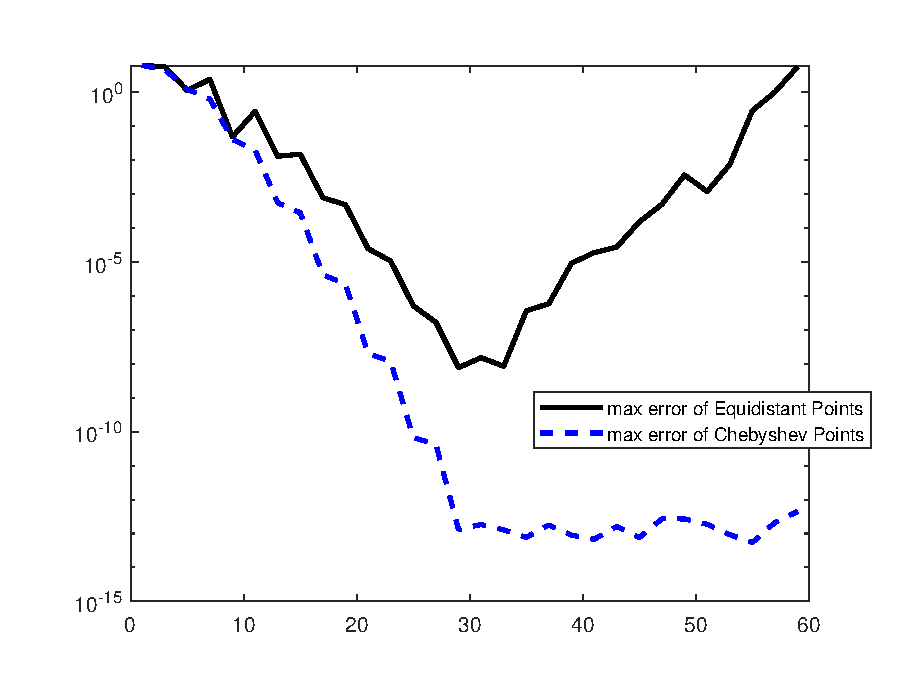
\includegraphics[width=0.7\textwidth]{image/T2_d.eps}
    \caption{第二题(d)小题作图结果}
\end{figure}
可以看到按照等距点插值的做法在点数增多到一定程度之后反倒其最大误差会急剧增大,而Chebyshev点不仅在等插值点数情况下其最大误差普遍更小,而且随着点数增多,即使接近50之前,其最大误差也尚未像等距插值一样大幅回升。

其原因在于等距点插值随着插值点数的增多,Runge现象在高阶情形下影响逐渐凸显,使得拟合的数值在拟合区间边缘出现较大的偏差,后者采用的是高阶而非等距的Chebyshev点,通过精心选取一系列在区间中心稀疏而在边缘密集的插值点,减少了Runge现象的影响,于是可以看到图中即使在n到达30以上的值后,依然尚为出现明显的Runge现象,即如等距插值那般出现由于区间边缘误差突然增长而最大误差值陡然回升的情况。

\textbf{第三题} 

(a)积分区间$[x_{n-1}, x_{n+1}]$,积分结点$\left\{x_{n+1},x_n,x_{n-1},x_{n-2}\right\}$\\
记$\alpha=ha_0,\beta=ha_1,\gamma=ha_2,\mu=ha_3$,于是有
\begin{equation}
    a_0h=\int_{x_{n-1}}^{x_{n+1}} \frac{(x-x_n)(x-x_{n-1})(x-x_{n-2})}{(x_{n+1}-x_n)(x_{n+1}-x_{n-1})(x_{n+1}-x_{n-2})}\, dx =\frac{1}{3}h \nonumber
\end{equation}
同理得,$a_1h=\frac{4}{3}h$,$a_2h=\frac{1}{3}h$,$a_3h=0$。\\
故得到公式
\begin{equation}
    y_{n+1}=y_{n-1}+\frac{h}{3}(f_{n+1}+4f_n+f_{n-1}+0f_{n-2}) \nonumber
\end{equation}

(b)展开得
\begin{equation}
    \begin{aligned}
        y_{n+1}&=y(x_{n-1})+\frac{h}{3}(f(x_{n+1},y(x_{n+1}))+4f(x_n,y(x_n))+f(x_{n-1},y(x_{n-1}))) \\
                &=y(x_{n-1})+\frac{h}{3}(y'(x_{n+1})+4y'(x_n)+y'(x_{n-1}))
    \end{aligned}
    \nonumber
\end{equation}
比较得局部截断误差,
\begin{equation}
    T_{n+1}=\int_{x_{n-1}}^{x_{n+1}}\frac{y^{(5)}(\xi)}{5!}(x-x_{n+1})(x-x_n)(x-x_{n-1})(x-x_{n-2})dx = O(h^5) \nonumber
\end{equation}
故公式为4阶

(c)由前面所得公式结合题目函数,直接得到其递推式
\begin{equation}
    y_{n+1} = (y_{n-1} + \frac{h}{3}(x_{n-1}e^{-5x_{n-1}}+4x_ne^{-5x_n}+x_{n+1}e^{-5x_{n+1}}-5y_{n-1}-20y_n)) \bigg/ (1+\frac{5h}{3}) \nonumber
\end{equation}
显然,我们所使用的多步法本身就是四阶的,为了不影响格式的整体截断误差,起步计算的格式精度至多只能比该格式的精度低一阶,即至少需要用三阶以上精度的格式来计算,而三阶的RungeKutta方法作为三阶格式恰满足其要求。\\
籍此可书写代码进行计算
\begin{lstlisting}[frame=single]
clear ,clc , clf
LW = 'linewidth';lw = 2;

% Def of the problem
n = 100;
F = @(x)(x.^2).*exp(-5.*x)/2;
a = 0;b = 2;

% Init Case
x = linspace(a,b,n+1);
y = zeros(1,n+1);
h = (b - a) / n;

% for error
f = F(x);

%%
% RK-3 Calculate
y(1) = 0;
y(2) = RK_3(h,x(1),y(1));
y(3) = RK_3(h,x(2),y(2));
%%
% Multi-Step Calculate
for i = 3:n
    y(i+1) = (y(i-1) + h*(x(i-1)*exp(-5*x(i-1)) +
            4*x(i)*exp(-5*x(i)) + x(i+1)*exp(-5*x(i+1)) -
            5*y(i-1) - 20*y(i)) / 3) /(1+5*h/3);
end
figure(1);
subplot(2,1,1);
p1 = plot(x,y,'b--',LW,lw);hold on
p2 = plot(x,f,'k',LW,lw);
legend([p1,p2],'approx','exact');
subplot(2,1,2);
p3 = plot(x,abs(f-y),'k',LW,lw);
legend(p3,'error','location','se');
%%
function y_next = RK_3(h,x_curr,y_curr)
    K1 = x_curr*exp(-5*x_curr)-5*y_curr;
    K2 = (x_curr + h/2)*exp(-5*(x_curr + h/2))-
            5*(y_curr + h*K1/2);
    K3 = (x_curr + h)*exp(-5*(x_curr + h))-
            5*(y_curr - h*K1 + 2*h*K2);
    y_next = y_curr + h*(K1+4*K2+K3)/6;
end
\end{lstlisting}
运行得到图6结果
\begin{figure}[htbp]
    \centering
    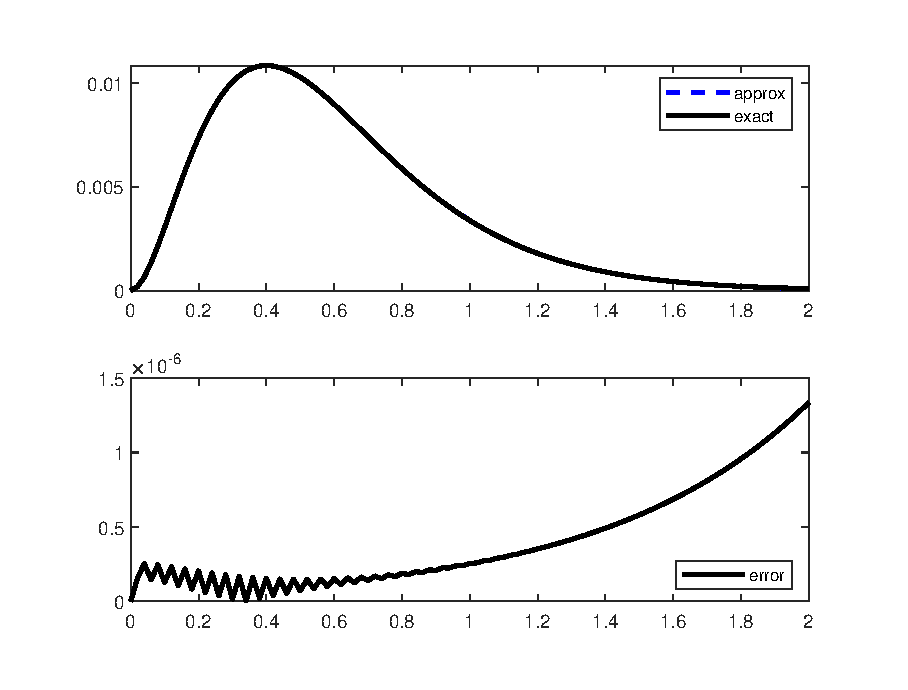
\includegraphics[width=0.7\textwidth]{image/T3_c.eps}
    \caption{第三题(c)小题作图结果}
\end{figure}

(d)解微分方程得其解为
\begin{equation}
    y = x^2\frac{e^{-5x}}{2} \nonumber
\end{equation}
据此编写代码计算得
\begin{lstlisting}[frame=single]
clear ,clc , clf
LW = 'linewidth';lw = 2;

% Def of the problem
F = @(x)(x.^2).*exp(-5.*x)/2;
a = 0;b = 2;

error_inf = 1e2; error_sup = 1e4;
error = zeros(1,error_sup)
for n = error_inf:error_sup
    error(n) = Multi_Step(F,a,b,n);
end
figure(1);
p1 = loglog((error_inf:error_sup),
        error(error_inf:error_sup),'k');
legend(p1,'error','location','se');
xlabel('n');
ylabel('误差');    
%%
function S = Multi_Step(F,a,b,n)
% Init Case
    x = linspace(a,b,n+1);
    y = zeros(1,n+1);
    h = (b - a) / n;

% for error
    f = F(x);

%%
% RK-3 Calculate
    y(1) = 0;
    y(2) = RK_3(h,x(1),y(1));
    y(3) = RK_3(h,x(2),y(2));
%%
% Multi-Step Calculate
    for i = 3:n
        y(i+1) = (y(i-1) + h*(x(i-1)*exp(-5*x(i-1)) +
                4*x(i)*exp(-5*x(i)) + x(i+1)*exp(-5*x(i+1)) -
                5*y(i-1) - 20*y(i)) / 3) /(1+5*h/3);
    end
%%
% Output
    S = max(abs(f-y));
end
%%
function y_next = RK_3(h,x_curr,y_curr)
    K1 = x_curr*exp(-5*x_curr)-5*y_curr;
    K2 = (x_curr + h/2)*exp(-5*(x_curr + h/2))-
            5*(y_curr + h*K1/2);
    K3 = (x_curr + h)*exp(-5*(x_curr + h))-
            5*(y_curr - h*K1 + 2*h*K2);
    y_next = y_curr + h*(K1+4*K2+K3)/6;
end
\end{lstlisting}
运行得到图7结果
\begin{figure}[htbp]
    \centering
    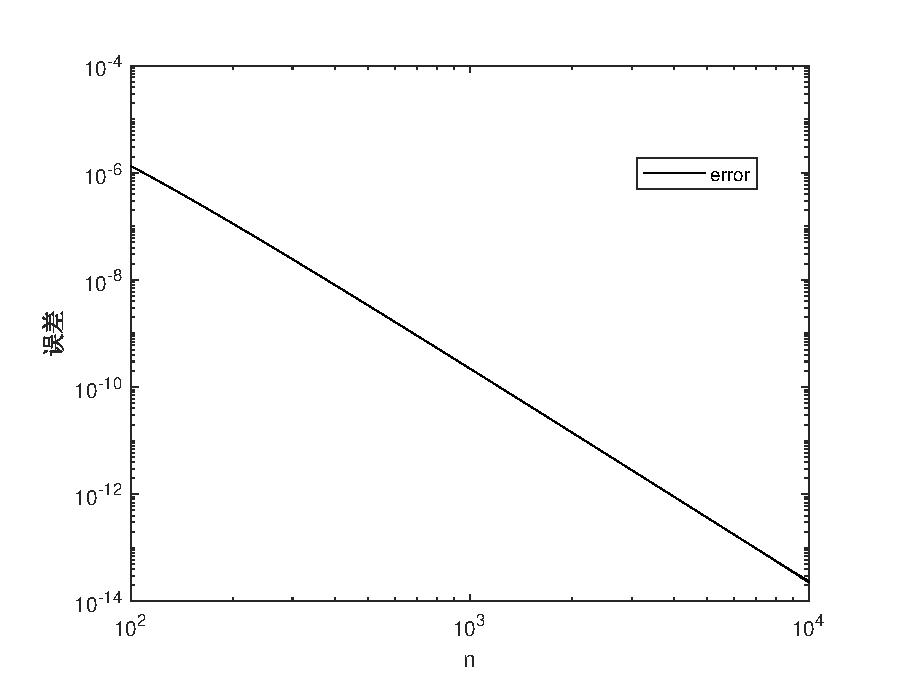
\includegraphics[width=0.7\textwidth]{image/T3_d.eps}
    \caption{第三题(d)小题作图结果}
\end{figure}
从图中不难看出其斜率为4,验证了先前对其公式为4阶的推论。
\end{enumerate}

\end{document}
